\documentclass{article}

\usepackage{amsfonts}
\usepackage{amsmath}
\usepackage{xcolor}
\usepackage{textcomp}
\usepackage{graphicx}
\usepackage{minted}

\title{ECE-210-A HW3}
\author{Instructor: Jonathan Lam}
\date{Spring 2022}

\begin{document}
\maketitle

\noindent This homework reviews indexing and functions as covered in class.

\begin{enumerate}
\item
  Let's look at images! This question uses \mintinline{matlab}|imshow| (see the help page!) and logical indexing to produce some simple shapes and show how we can use them as masks for image manipulation.
  
  \begin{enumerate}
  \item Create the logical matrix $A\in M_{256\times 256}(\mathbb{F}_2)$ where $a_{ij}$ is true iff $\sqrt{(i-128)^2+(j-128)^2}<64$. (Use \mintinline{matlab}|meshgrid| or broadcasting.)
    
    ($\mathbb{F}_2$, or Galois-field 2, is the field consisting of only the values $\{0,1\}$ and whose operations are akin to logical operators. For our purposes, these are the two logical values corresponding to false and true.)
    
  \item Create the logical matrix $B\in M_{256\times 256}(\mathbb{F}_2)$ where $b_{ij}$ is true iff $\sqrt{(i-96)^2+(j-96)^2}<64$.
    
  \item Create the following logical matrices. For each one, use \mintinline{matlab}|figure| and \mintinline{matlab}|imshow| to visualize it. Briefly describe each one in a comment.
    \begin{enumerate}
    \item $A$
    \item $B$
    \item $C=A\cap B^C$
    \item $D=A^C\cup B$
    \end{enumerate}
    
  \item Visualize the following matrices using \mintinline{matlab}|figure| and \mintinline{matlab}|imshow|. What do the \mintinline{matlab}|.*| and \mintinline{matlab}|+| operators do when dealing with logical arrays? (Think layer masks.)
\begin{minted}{matlab}
E = rand(256, 256, 3);
F = linspace(0, 0.25, 256) + linspace(0, 0.25, 256).';
G = E .* C + F .* D;
\end{minted}
    
  \item \textit{(Optional)} Rather than putting each plot in a new figure, use subplots using \mintinline{matlab}|subplot| or \mintinline{matlab}|tiledlayout|. Label each plot!
    
  \item \textit{(Optional)} Implement a function, \mintinline{matlab}|generate_circle(x, y, rad)| that takes in the coordinates of the circle's center and its radius, and generates a $256\times 256$ logical matrix, and use it for parts (a) and (b). Alternatively, use it to generate arbitrary circles and visually demonstrate the inclusion-exclusion principle by \mintinline{matlab}|xor|-ing all the circles.
  \end{enumerate}
  
  \clearpage
\item
  Calculus time!
  \begin{enumerate}
  \item Write a function \mintinline{matlab}|deriv(y, x)| and \mintinline{matlab}|antideriv(y, x)| which take vectors \mintinline{matlab}|y| and \mintinline{matlab}|x|, and which perform numerical differentiation and integration on the function $y=y(x)$. These should each output vectors of the same length as the input; you may need to pad your result with an arbitrary value. You did this already; now make it a function.
    
  \item Write a function \mintinline{matlab}|switchsign(x)| which takes a vector \mintinline{matlab}|x| and returns a logical array with the same length as \mintinline{matlab}|x| that is true when \mintinline{matlab}|x| switches sign. E.g., for \mintinline{matlab}|x=[2 3 -1 0 -1 5]| it would return \mintinline{matlab}|[0 0 1 0 0 1]|. Do not use a \mintinline{matlab}|for| loop.
    
    (Hint: One way to vectorize this is to use the \mintinline{matlab}|sign| and \mintinline{matlab}|diff| functions. Another way is to write conditions on the vector and use a shifted version of itself. You will probably need to pad the resulting vector to make it the same length as the original vector; one way to do this is to repeat the first element of the resulting vector twice.)
    
  \item Write a function \mintinline{matlab}|extrema(y, x)| that uses the first derivative test to find local extrema (minima and maxima). Recall that local extrema on a differentiable function occur when $y'(x)$ changes sign. Use your \mintinline{matlab}|deriv| and \mintinline{matlab}|switchsign| functions here. The output of this function should also be two vectors: one representing the $y$ values of the extrema, and one representing the corresponding $x$ values.
    
  \item Write a function \mintinline{matlab}|inflections(y, x)| that uses the second derivative test to find inflection points (i.e., when $y''(x)$ changes sign).
    
  \item Let $x$ be a 1001-point vector linearly spaced from $-2\pi$ to $2\pi$. Use \mintinline{matlab}|sinc| to generate $y=\text{sinc}(x)$ over this interval. Generate the following variables using the functions you just wrote:
    \begin{enumerate}
    \item \mintinline{matlab}|y_antideriv|, the antiderivative of $y$
    \item \mintinline{matlab}|y_deriv|, the derivative of $y$
    \item \mintinline{matlab}|y_extr| and \mintinline{matlab}|x_extr|, the coordinates of the local extrema of $y$
    \item \mintinline{matlab}|y_infl| and \mintinline{matlab}|x_infl|, the coordinates of the inflection points of $y$
    \end{enumerate}
    Plot these using: \begin{minted}{matlab}
plot(x,y,x,y_antideriv,x,y_deriv, ...
     x_extr,y_extr,'r*',x_infl,y_infl,'bo');
\end{minted}
    Title your plot and label the axes. It should look something like:
    \begin{figure}[!h]
      \centering
      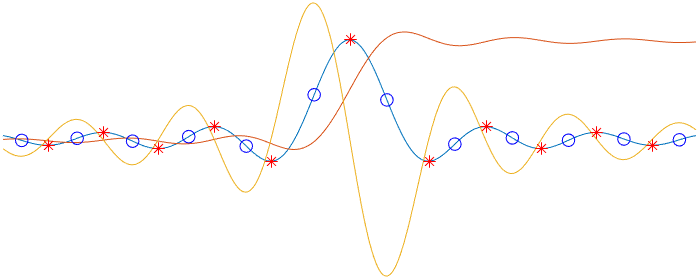
\includegraphics[width=2.5in]{result.png}
    \end{figure}
  \end{enumerate}
\end{enumerate}

\end{document}
%%% Local Variables:
%%% mode: latex
%%% TeX-master: t
%%% End:
